\subsection{Conservation, fields, and physical models across scales -- study additions}
\label{study-physics}
\textit{AI-assisted editorial study additions: original explanations and illustrations, not verbatim historical writing nor a transcript. These are high-level bridges to the detailed source notes, not a reconstruction of every course or derivation.}

\subsubsection{Newtonian and Lagrangian mechanics}
Start by specifying the system boundary, coordinates, inertial frame, constraints, and applied forces. Newton's law $d p/dt=F_{\mathrm{ext}}$ reduces to $m\ddot x=F$ for constant mass; variable-mass systems require accounting for momentum flux. Work changes kinetic energy, while an interaction potential exists only when the force is conservative in the relevant configuration domain. Conservation of total energy includes heat and internal energy, not merely visible mechanical motion.

For generalized coordinates $q_i$, write $L=T-V$ and
\begin{equation}
\frac{d}{dt}\frac{\partial L}{\partial\dot q_i}-\frac{\partial L}{\partial q_i}=Q_i.
\label{study-physics-lagrange}
\end{equation}
Here $Q_i$ represents nonconservative generalized forces. Time-translation symmetry gives conserved energy; spatial and rotational symmetry give momentum and angular momentum under the appropriate isolated-system assumptions. A cyclic coordinate yields conserved conjugate momentum even when that momentum is not simply mass times coordinate velocity. Constraints can simplify coordinates without doing work, but friction and moving constraints need explicit treatment.

For a spring-mass-damper, $m\ddot x+c\dot x+kx=0$. Define $\omega_0=\sqrt{k/m}$ and $\zeta=c/(2\sqrt{km})$. With $m,k>0$ and $c>0$, mechanical energy obeys $\dot E=-c\dot x^2$. Underdamped motion oscillates while losing energy; critical damping separates oscillatory and nonoscillatory regimes. Resonant forced response depends on damping and on which observable is measured. Section~\ref{study-control} reinterprets these modes as poles rather than introducing different physics.
\begin{figure}[htbp]
\centering
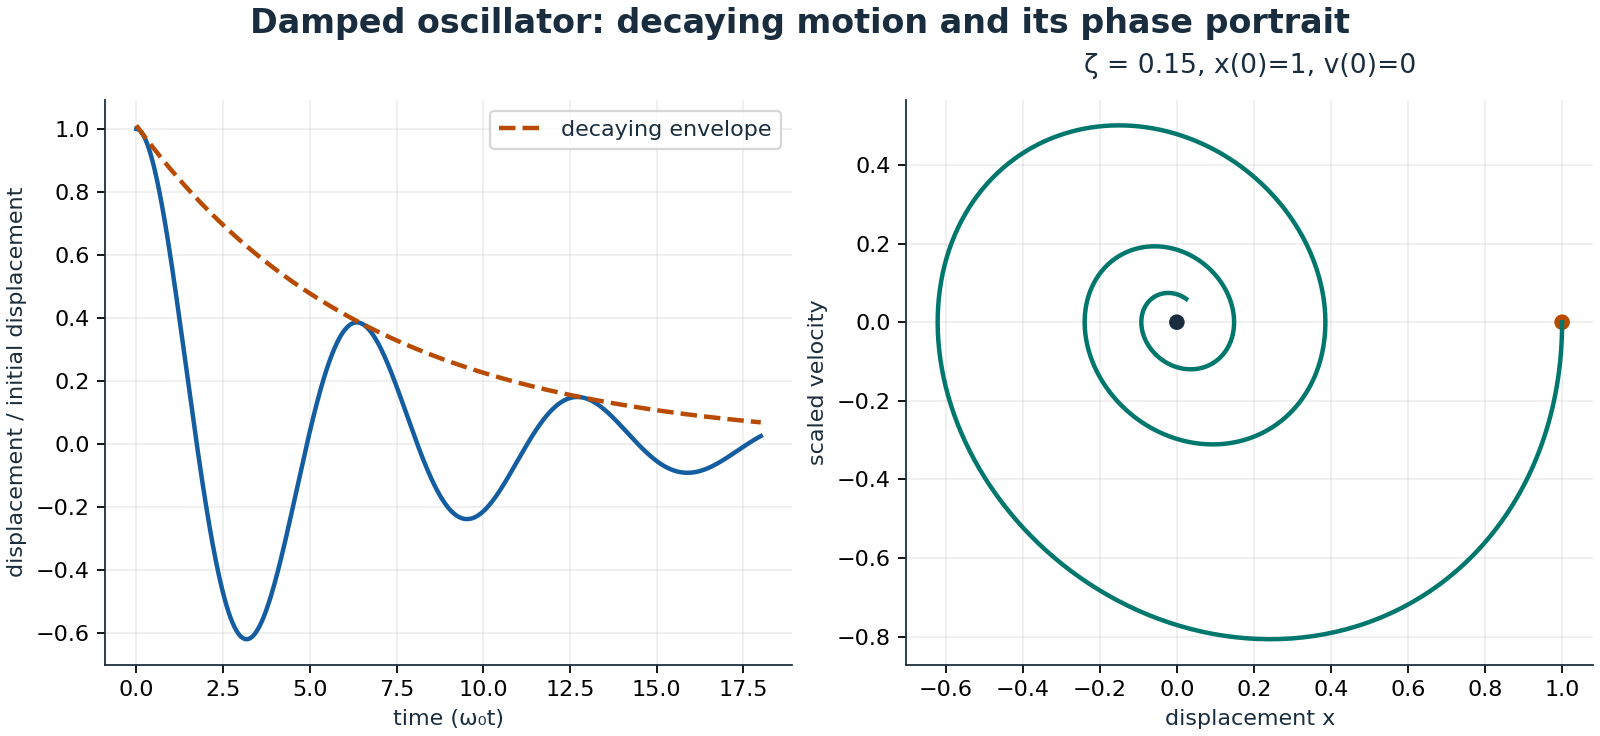
\includegraphics[width=0.95\linewidth]{tex_images/mental_map/study/physics_oscillator.png}
\caption{Exact unforced underdamped motion with normalized natural frequency one, damping ratio 0.15, and zero initial velocity. The phase trajectory spirals inward because mechanical energy is dissipated.}
\end{figure}

\subsubsection{Waves and optics}
The one-dimensional wave equation $u_{tt}=v^2u_{xx}$ supports travelling disturbances, while boundaries select standing modes. Phase velocity describes a constant-phase point; group velocity $d\omega/dk$ describes a narrowband envelope when dispersion is mild enough. Superposition applies to the linear model, not automatically to high-amplitude waves. Intensity is quadratic in field amplitude, so coherent waves interfere before intensities are computed.

Snell's law $n_1\sin\theta_1=n_2\sin\theta_2$ uses angles from the normal. Geometrical rays neglect diffraction and require lengths large relative to wavelength. For equal coherent slits of width $a$ separated by $d$, far-field intensity is proportional to $[\sin\beta/\beta]^2\cos^2\delta$, with $\beta=\pi a\sin\theta/\lambda$ and $\delta=\pi d\sin\theta/\lambda$. Finite aperture sets the envelope; separation sets fine fringes. Resolution is limited by wavelength, aperture, aberrations, and noise, not magnification alone.
\begin{figure}[htbp]
\centering
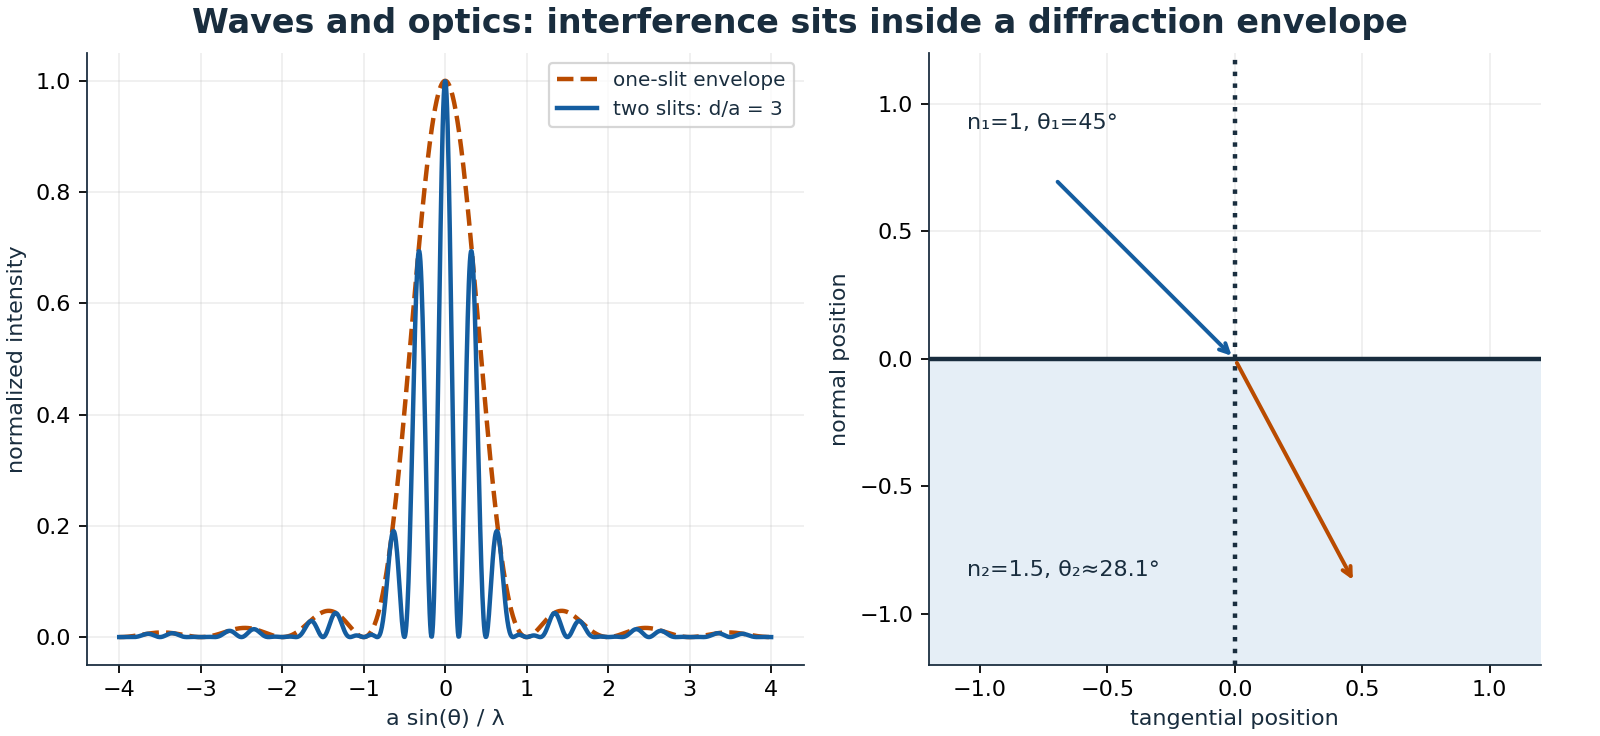
\includegraphics[width=0.95\linewidth]{tex_images/mental_map/study/physics_optics.png}
\caption{Fraunhofer two-slit intensity for separation three slit widths, and refraction from index one to 1.5. The ray drawing is schematic; the intensity assumes monochromatic coherent illumination.}
\end{figure}

\subsubsection{Continuum mechanics, dimensions, and boundaries}
A continuum averages over microscopic structure. It is useful only when the observation scale supports that averaging. Displacement $u$ gives infinitesimal strain $\epsilon=(\nabla u+\nabla u^T)/2$ when rotations and deformation gradients are sufficiently small. Stress is force per area: traction on normal $n$ is $t=\sigma n$. Stress symmetry follows from angular-momentum balance for an ordinary continuum without couple stresses. Linear isotropic elasticity uses $\sigma=\lambda\operatorname{tr}(\epsilon)I+2\mu\epsilon$; anisotropic crystals require a stiffness tensor.

For an incompressible Newtonian fluid of constant density and viscosity,
\begin{equation}
\rho(\partial_t v+v\cdot\nabla v)=-\nabla p+\mu\nabla^2v+\rho b,
\qquad\nabla\cdot v=0.
\label{study-physics-fluid}
\end{equation}
Each momentum term has units of force per volume. The Reynolds number $\rho UL/\mu$ compares inertial and viscous effects, but a single universal transition value does not exist for all geometries. No-slip at a stationary wall produces a parabolic fully developed pressure-driven channel profile. At rarefied or molecular scales, slip and noncontinuum transport can invalidate that boundary model.
\begin{figure}[htbp]
\centering
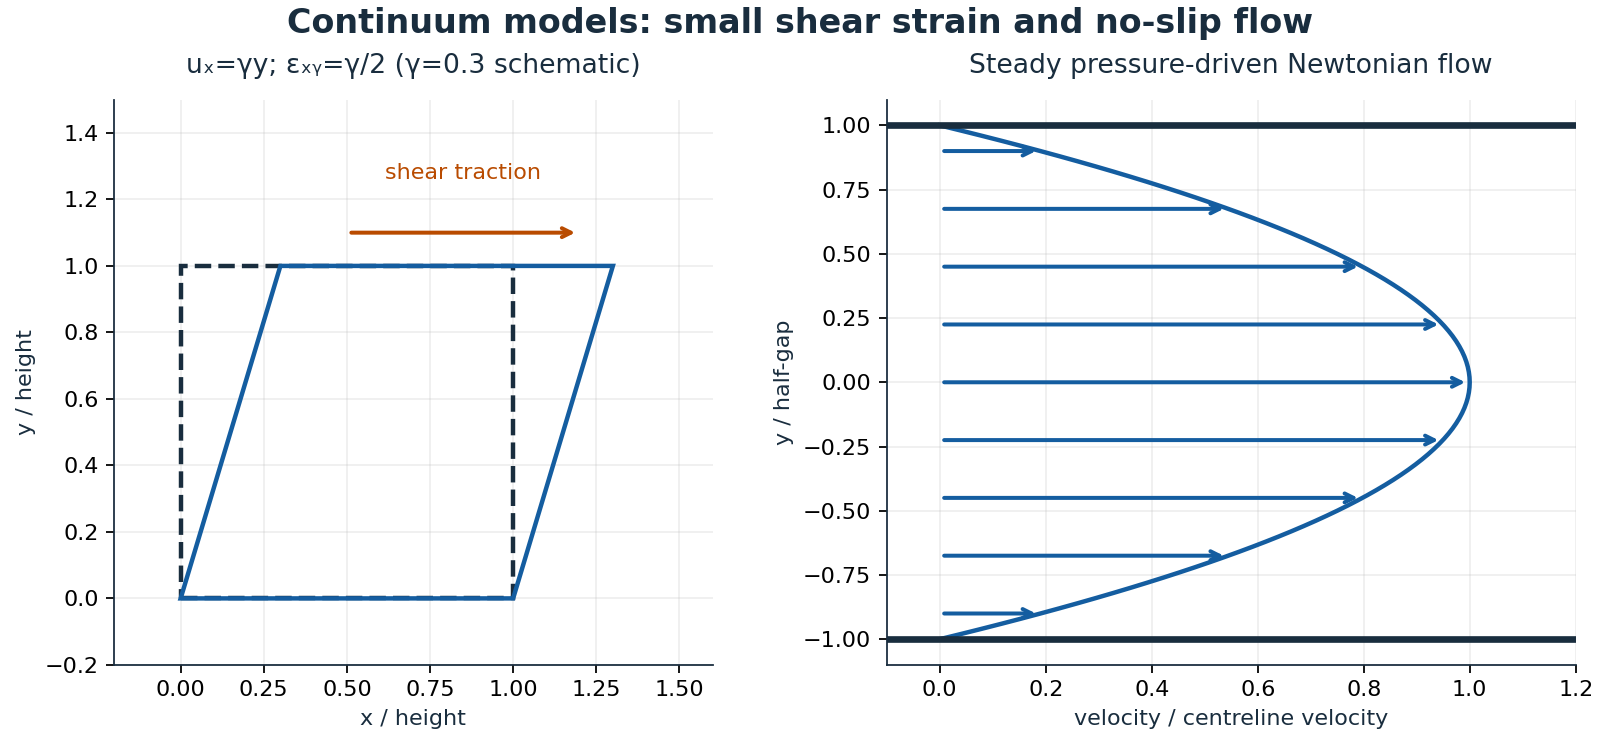
\includegraphics[width=0.95\linewidth]{tex_images/mental_map/study/physics_continuum.png}
\caption{Simple shear illustrates the factor of two between engineering shear and tensor shear strain; the exaggerated deformation is schematic. The channel solution assumes steady laminar incompressible flow between stationary parallel walls.}
\end{figure}

With constant properties, conduction satisfies $\rho c_p\partial_t T=k\nabla^2T+\dot q$, where $\dot q$ is volumetric heating. Thermal diffusivity $\alpha=k/(\rho c_p)$ has dimensions length squared per time, giving diffusion time $L^2/\alpha$. Dirichlet data prescribe temperature; Neumann data prescribe normal flux; Robin data couple flux to environmental temperature, for example $-k\partial_nT=h(T-T_\infty)$. Sign depends on the outward normal convention. Initial and boundary data are part of the problem, not numerical afterthoughts.
\begin{figure}[htbp]
\centering
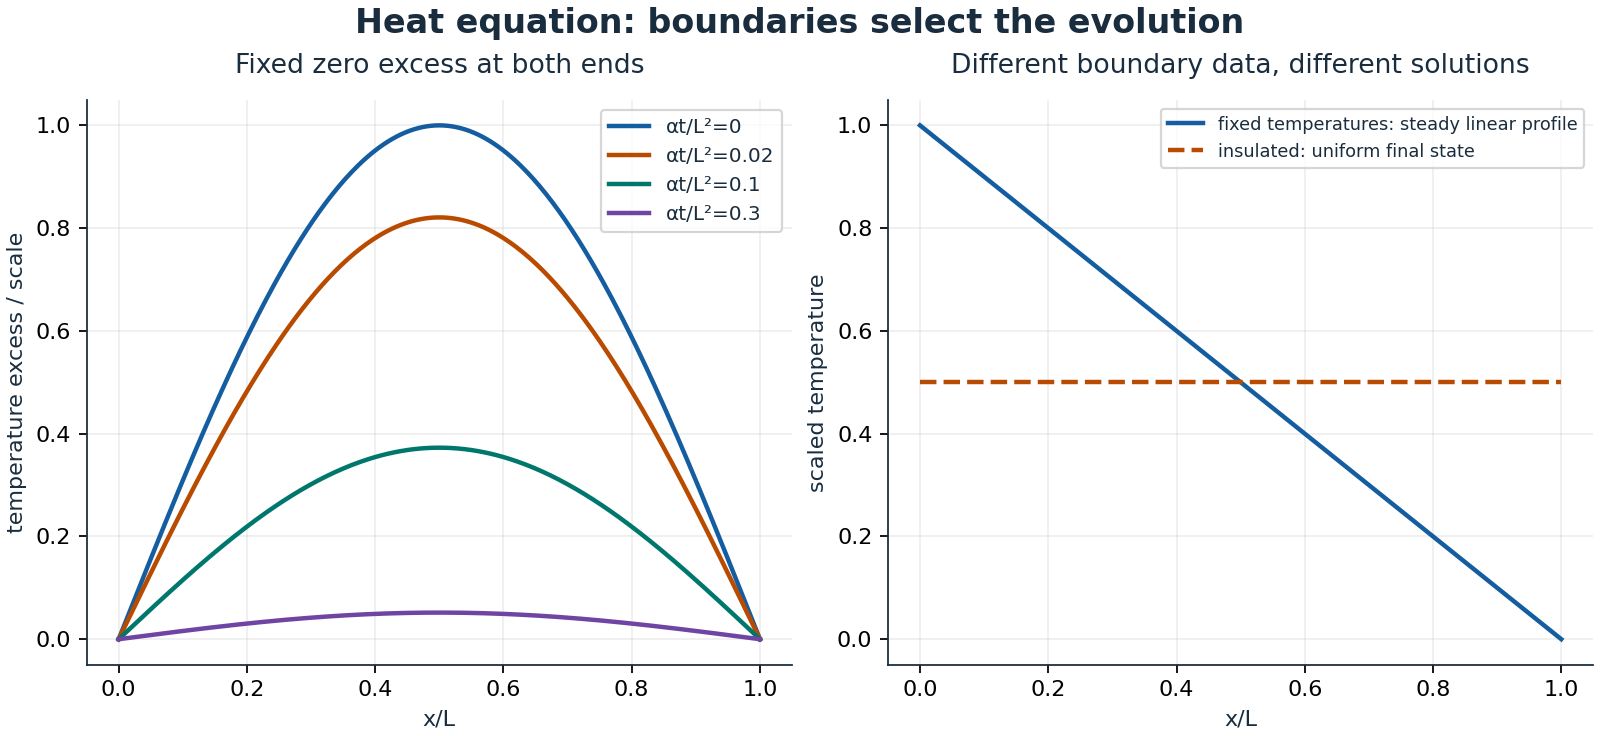
\includegraphics[width=0.95\linewidth]{tex_images/mental_map/study/physics_heat.png}
\caption{An exact decaying sine mode with fixed endpoint temperature excess, alongside schematic steady profiles for fixed temperatures and insulated boundaries. The insulated final temperature is determined by conserved total heat.}
\end{figure}

\subsubsection{Maxwell fields, circuits, and carriers}
Macroscopic Maxwell equations relate free charge and current to fields:
\begin{align}
\nabla\cdot D&=\rho_f,&\nabla\cdot B&=0,\\
\nabla\times E&=-\partial_t B,&\nabla\times H&=J_f+\partial_tD.
\end{align}
Constitutive relations such as $D=\epsilon E$ and $B=\mu H$ add material assumptions. Displacement current preserves charge continuity. The Poynting vector $E\times H$ describes electromagnetic energy flux. Integral statements connect to the flux and circulation diagrams in Section~\ref{study-math}.

Lumped circuits approximate spatially distributed fields when propagation delays and geometry allow. Kirchhoff's current law expresses charge balance; the usual loop law neglects unmodelled changing magnetic flux. Using the $e^{j\omega t}$ convention, $Z_R=R$, $Z_L=j\omega L$, and $Z_C=1/(j\omega C)$. State whether phasors use peak or RMS amplitude before calculating average power. In semiconductors, conductivity depends on mobile electrons and holes, their concentrations, and mobilities. Doping changes carrier statistics; the junction discussion in Section~\ref{study-nano} distinguishes moving carriers from fixed ionized dopants.
\begin{figure}[htbp]
\centering
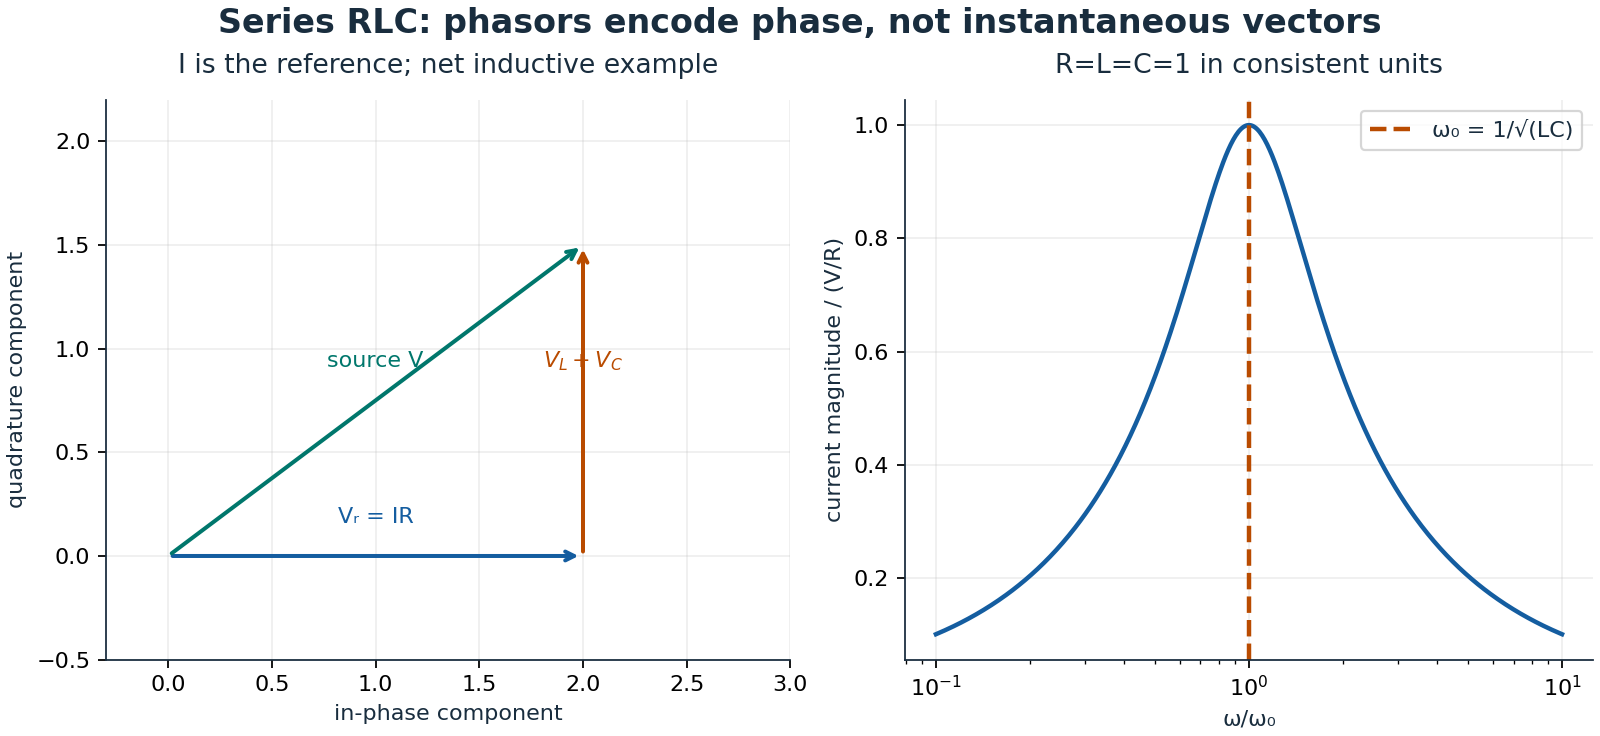
\includegraphics[width=0.95\linewidth]{tex_images/mental_map/study/physics_phasor.png}
\caption{Series-RLC voltage addition with current as phase reference, and normalized current resonance for consistent unit component values. The phasor triangle is illustrative, not a physical spatial orientation of circuit elements.}
\end{figure}

\subsubsection{Quantum states, ensembles, and relativity bridges}
A normalized wavefunction supplies probabilities, not a hidden classical trajectory. In an infinite one-dimensional box, $\psi_n=\sqrt{2/L}\sin(n\pi x/L)$ and $E_n=n^2\pi^2\hbar^2/(2mL^2)$ for positive integers $n$. Narrower confinement raises kinetic energy. The harmonic oscillator has $E_n=\hbar\omega(n+1/2)$ and nonzero ground energy. These are different potentials with different level spacings; neither spacing is universal.
\begin{figure}[htbp]
\centering
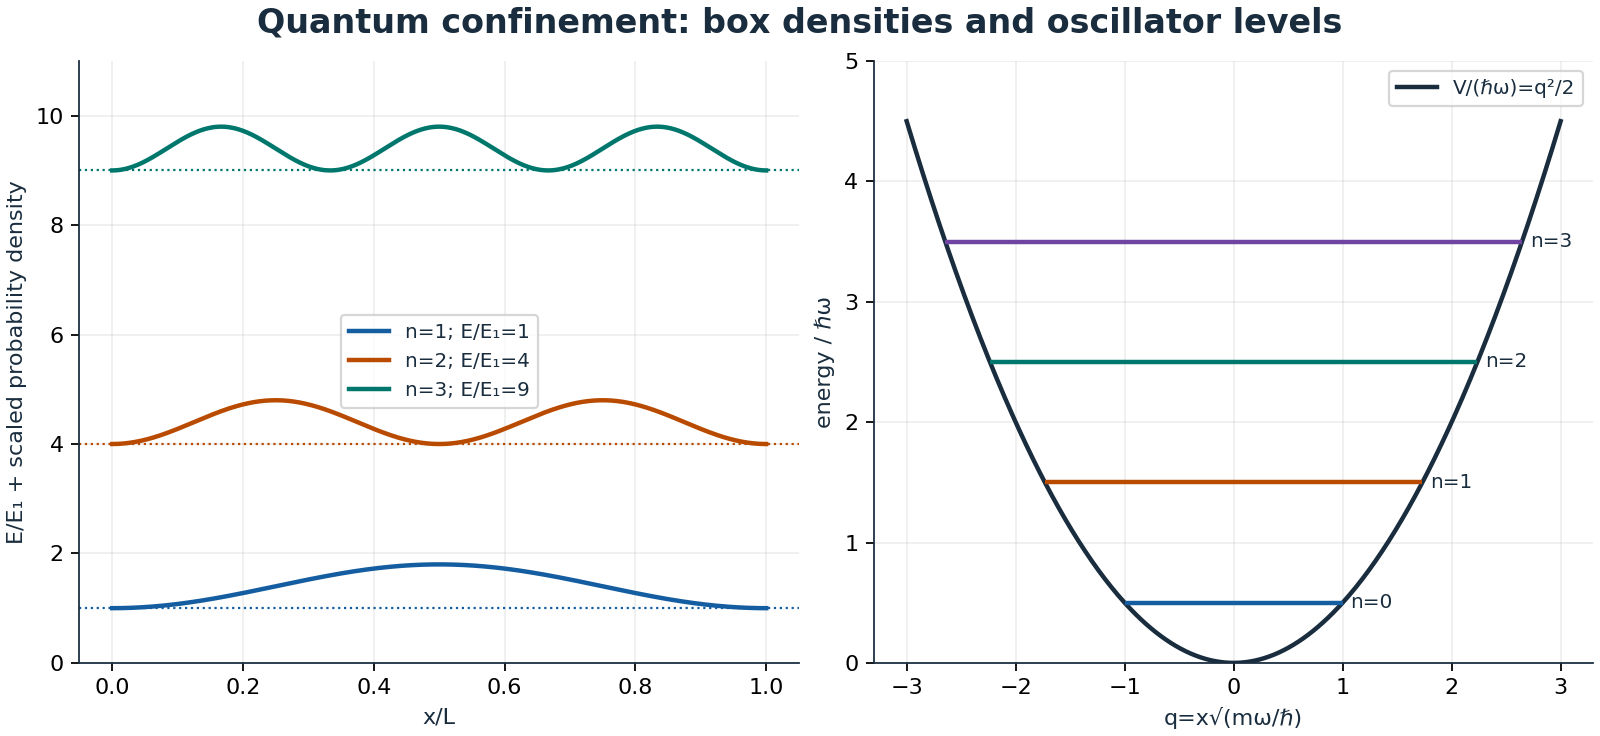
\includegraphics[width=0.95\linewidth]{tex_images/mental_map/study/physics_quantum.png}
\caption{Box probability densities are vertically offset by their energies; their plotted height is not an energy correction. Harmonic-oscillator levels have equal spacing and classical turning-point endpoints in a quadratic potential.}
\end{figure}

Angular momentum obeys $[L_x,L_y]=i\hbar L_z$, with $L^2=\hbar^2\ell(\ell+1)$ and $L_z=m\hbar$ on joint eigenstates. Orbital $\ell$ is integer; spin requires its own representation and may be half-integer. The uncertainty relation reflects noncommuting observables, not merely imperfect instruments. A pure superposition and a statistical mixture can share some measurement probabilities while differing in coherence.

The canonical ensemble fixes temperature, volume, and particle number, assigning $p_i=e^{-\beta E_i}/Z$. The grand canonical ensemble permits particle exchange and weights $E_i-\mu N_i$. Entropy connects microstate probabilities to thermodynamics; quantum indistinguishability distinguishes Bose and Fermi statistics. Finally, special relativity replaces absolute time with invariant spacetime interval and $E^2=p^2c^2+m^2c^4$. Newtonian mechanics emerges at low speed; general relativity further treats gravitation geometrically. These bridges orient the detailed quantum and statistical notes rather than replacing their derivations.

\subsubsection{Sources and scope}
See \href{https://openstax.org/details/books/university-physics-volume-1}{OpenStax University Physics, Volume 1}, \href{https://openstax.org/details/books/university-physics-volume-2}{Volume 2}, and \href{https://openstax.org/details/books/university-physics-volume-3}{Volume 3}. The \href{https://ucalendar.uwaterloo.ca/2223/COURSE/course-NE.html}{Waterloo 2022/23 NE descriptions} guide topics associated with mechanics, continuum models, electromagnetism, quantum mechanics, and statistical thermodynamics; this is a scope map, not evidence of completed courses.